\documentclass{beamer}
\usepackage[ngerman]{babel}
\usepackage[utf8]{inputenc}
\usepackage{amsmath}
\usepackage{amsthm}
\usepackage{siunitx}
\usepackage{graphicx}
\usepackage{pgfplots}
\sisetup{locale = DE}
% Lade Beamer Stile
\usepackage{beamerthemesplit}
\usepackage{tcolorbox}
\usetheme{Rochester}
\usecolortheme{crane}

\usepackage{wrapfig}
\usepackage{multicol}
\usepackage{xcolor}
\newcolumntype{C}[1]{>{\centering\arraybackslash}p{#1}@{}}

\title{3. Unterrichtseinheit zur Wärmelehre}
\subtitle{Wärmeenergie}
\author{Heiko Schröter}
\date{\today}
\titlegraphic{
\includegraphics[scale=0.6]{logo_RHS.pdf}}
\setbeamertemplate{enumerate item}{\alph{enumi})}

\begin{document}

\frame{\titlepage}

\frame
{
  \frametitle{Ziele für die heutige Unterrichtseinheit}
  \textbf{Was verstehen wir unter Wärmeenergie und Wärmemenge?}
  \begin{itemize}
	\item Was versteht man unter dem absoluten Nullpunkt, wie ist dieser energetisch gekennzeichnet?
	\item Wovon hängt die Längenausdehnung eines Körpers ab?
	\item Welcher Zusammenhang liegt zwischen der Längenausdehnung und der Volumenausdehnung vor?
	\item Warum ist Wasser als Ausdehnungsflüssigkeit in einem Flüssigkeitsthermometer ungeeignet?
	\item Welche Druckkraft resultiert aus der Erwärmung einer fest eingebauten Rohrleitung?
  \end{itemize}
}

\frame
{
  \frametitle{Wärmelehre Begriffsbestimmung}
\begin{large}
  \begin{center}
  \textbf{Temperatur, innere Energie, Wärme}
  \end{center}
\end{large}
\begin{small}
  \begin{tabular}{p{2.8cm}p{3cm}p{4cm}}
  \textbf{Temperatur $T$} & \textbf{innere Energie $E_i$} & \textbf{Wärme $Q$} \\
  gibt an, wie kalt oder warm ein Körper ist. & gibt an, welche Energie ein Körper aufgrund seiner Temperatur hat. & gibt an, wie viel thermische Energie von einem Körper auf einen anderen übertragen wird. \\ 
  \end{tabular} 
\end{small}
  \begin{tikzpicture}
  \begin{scope}[scale=0.03]
  \begin{footnotesize}
    \filldraw [color=red, fill=orange, thick] (0,0) -- (50,0) -- (50,50) -- (0,50) -- cycle;
    \filldraw [color=black, fill=lightgray, thick] (250,0) -- (300,0) -- (300,50) -- (250,50) -- cycle;
    \draw [->, >=latex, thick, black] (-20,45) -- (-20,0) node [midway, right] {$E_i$};
    \draw [->, >=latex, thick, black] (320,5) -- (320,50) node [midway, right] {$E_i$};
	\node (T1) at (25,25) {Körper 1};
	\node (T2) at (275,25) {Körper 2};
    \fill [color=black, fill=lightgray] (50,5) -- (230,20) -- (230,15) -- (250,25) -- (230,35) -- (230,30) -- (50,45) -- cycle;
    \node (T) at (120,25) {Wärme $Q=\Delta E_i$};
    \node (T11) at (25,60) {hohe Temperatur};
    \node (T12) at (25,-10) {Temperatur sinkt};
    \node (T21) at (275,60) {niedrige Temperatur};
    \node (T22) at (275,-10) {Temperatur steigt};
  \end{footnotesize}
  \end{scope}
  \end{tikzpicture}
}

\frame[allowframebreaks]
{
  \frametitle{Der Mechanismus der Wärmespeicherung}
  \begin{block}{Wärmeenergie (innere Energie}
  Bei Zuführung von Wärmeenergie erhöht sich die Bewegungsenergie der Elementarbausteine und umgekehrt nimmt diese bei Wärmeabfuhr ab.
  \end{block}
Obwohl jede Zuführung von Wärmeenergie die Bewegungsenergie der Moleküle vergrößert, ist feststellbar, dass es einen grundsätzlichen Unterschied gibt:
  \begin{block}{sensible Wärme $\rightarrow$}
  Die zu- oder abgeführte Energie ändert die Körpertemperatur.
  \end{block}
  \newpage
  \begin{block}{latente Wärme $\rightarrow$}
  \textbf{versteckte Wärme} $\rightarrow$ Die zu- oder abgeführte Energie ändert den Aggregatzustand oder die Gitterstruktur des Körpers bei konstanter Temperatur. 
  \end{block}
\begin{figure}
	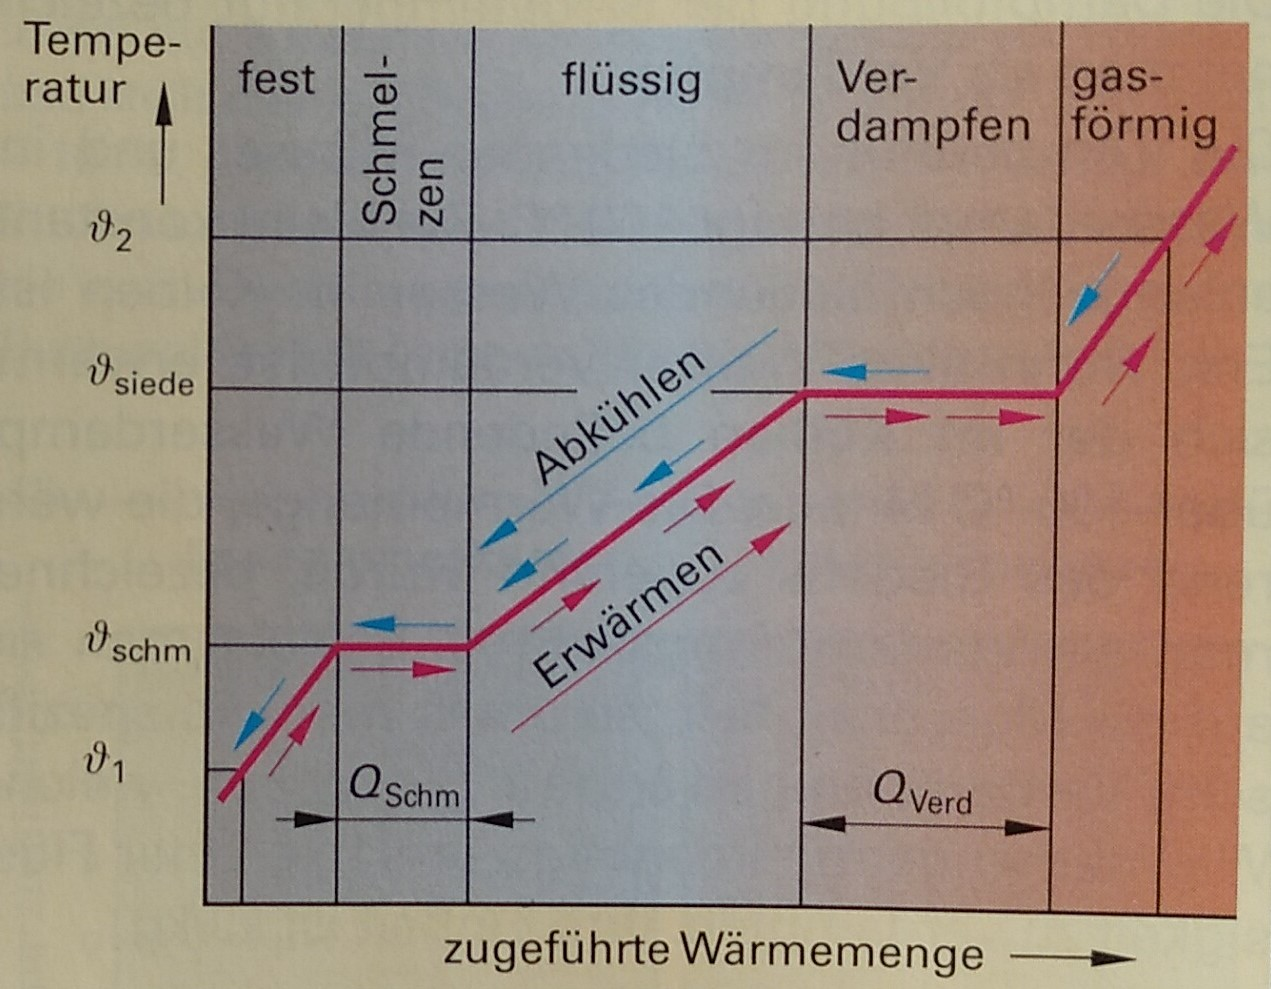
\includegraphics[width=.4\linewidth]{Temperaturkurve}
	\caption{Temperaturverlauf bei Wärmezufuhr bzw. Wärmeabfuhr}
\end{figure}
}

\frame[allowframebreaks]
{
  \frametitle{Wärmeenergie und absoluter Nullpunkt}
  \begin{block}{}
  Am absoluten Nullpunkt hat die Bewegungsenergie der Atome bzw. Moleküle ihren kleinst möglichen Wert.
  \end{block}
\begin{tabular}{@{} *{2}{C{.5\linewidth}} }
  \includegraphics[width=.55\linewidth]{Wärmebewegung_F.jpg} &
    \includegraphics[width=.55\linewidth]{Wärmebewegung_G.jpg} \\[\abovecaptionskip]
\end{tabular}
 \begin{center}
  Molekulare Wärmebewegung
 \end{center}
\newpage
  \begin{block}{3. Hauptsatz der Thermodynamik}
  Der absolute Nullpunkt kann niemals erreicht werden.
  \end{block}
Diese Aussage aus dem Jahr 1906 wurde von Max Planck in der Quantentheorie bestätigt. Experimentell ist man heute in der Lage, sich dem absoluten Nullpunkt bis auf weniger als $10^{-6}\si{\kelvin}$ zu nähern.
}

\frame
{
  \frametitle{Körper bei Wärmezufuhr oder Wärmeabgabe}
	\begin{scriptsize}	
	Wird einem Körper Wärme zugeführt oder von ihm Wärme abgegeben, so kann das verschiedene Auswirkungen haben.
	\begin{columns}
		\begin{column}{0.5\textwidth}
   			\begin{tcolorbox}
   			Die Temperatur des Körpers ändert sich.
	  		\begin{align*}
	  		&\Delta T=\dfrac{Q}{c\cdot m}\\
	  		&Q=c\cdot m\cdot\Delta T&
	  		\end{align*}
			\end{tcolorbox}
		\end{column}
		\begin{column}{0.5\textwidth}
     		\begin{tcolorbox}
	  		Bei der Umwandlungstemperatur ändert sich der Aggregatzustand.
	  		\begin{align*}
	  		&Q_s=m\cdot q_s\\
	  		&Q_v=m\cdot q_v&
	  		\end{align*}
			\end{tcolorbox}
   		\end{column}
		\end{columns}
			\vspace{0.3cm}	  		
	  		\centering \colorbox{lightgray}{{\normalsize Wärmezufuhr oder Wärmeabgabe}}
	\begin{columns}
		\begin{column}{0.5\textwidth}
   			\begin{tcolorbox}
	  		Volumen bzw. Länge des Körpers ändert sich.
	  		\begin{align*}
	  		&\Delta V=\gamma\cdot V_0\cdot\Delta T\\
	  		&\Delta l=\alpha\cdot l_0\cdot\Delta T&
	  		\end{align*}	  		
			\end{tcolorbox}
		\end{column}
		\begin{column}{0.5\textwidth}
     		\begin{tcolorbox}
	  		Die innere Energie das Körpers ändert sich. Es wird Wärme ausgetauscht oder Arbeit verrichtet.
	  		\begin{align*}
	  		&\Delta E_i=W+Q&
	  		\end{align*}   		
			\end{tcolorbox}
   		\end{column}
	\end{columns}
	\end{scriptsize}
}

\frame
{
  \frametitle{Wärmeausdehnung fester Körper}
  \begin{block}{}
  Die Volumenänderung infolge einer Temperaturänderung beruht auf der Änderung der Bewegungsenergie und damit der Änderung der Schwingungsweite der Atome.
  \end{block}
  \begin{block}{thermischer Längenausdehnungskoeffizient}
  Der thermische Längenausdehnungskoeffizient $\alpha$ ist stoffabhängig und temperaturabhängig. Er wird auch als Wärmedehnzahl oder linearer Ausdehnungskoeffizient bezeichnet.
  \end{block}
Die Einheit von $\alpha$ ist: 
	\begin{tcolorbox}	  
	  $\frac{m}{m\cdot \si{\celsius}} = \frac{m}{m\cdot K} = \frac{1}{K}$
	\end{tcolorbox}
}

\frame
{
	\begin{block}{Berechnung der Längenausdehnung infolge einer Temperaturdifferenz}
	\begin{align*}
	\Delta l&=l_1\cdot\alpha\cdot\Delta\vartheta &\rightarrow&\text{Wärmeausdehnung}\\
	l_2&=l_1\pm l_1\cdot\alpha\cdot\Delta\vartheta &\rightarrow&\text{Endlänge}
	\end{align*}
	\end{block}
	
}

\frame[allowframebreaks]
{
  \frametitle{Beispielaufgabe 1}
Eine Stahlschiene hat bei $\SI{10}{\celsius}$ eine Länge von $\SI{25}{\meter}$. Welche Länge hat die Schiene bei $\alpha=\SI{0.000012}{\frac{\meter}{\meter\kelvin}}$\\
\begin{enumerate}[a)]
\item im Sommer bei $\SI{40}{\celsius}$
\item im Winter bei $-\SI{5}{\celsius}$
\item Wie groß ist der gesamte Dehnbereich?
\end{enumerate}
\textbf{Lösung:}
\begin{enumerate}[a)]
\item \begin{align*}
	l_2&=l_1+l_1\cdot\alpha\cdot\Delta\vartheta=\SI{25}{\meter}+\SI{25}{\meter}\cdot\SI{0.000012}{\frac{\meter}{\meter\kelvin}}\cdot\SI{30}{\kelvin}\\&=\SI{25,009}{\meter}
	\end{align*}
\item \begin{align*}
	l_2&=l_1-l_1\cdot\alpha\cdot\Delta\vartheta=\SI{25}{\meter}-\SI{25}{\meter}\cdot\SI{0.000012}{\frac{\meter}{\meter\kelvin}}\cdot\SI{15}{\kelvin}\\&=\SI{24,9955}{\meter}
	\end{align*}
\item Der gesamte \textbf{Dehnbereich} zwischen $-\SI{5}{\celsius}$ und $\SI{40}{\celsius}$ beträgt somit $\Delta l_{ges}=\SI{13,5}{\milli\meter}$
\end{enumerate}
}

\frame[allowframebreaks]
{
\frametitle{Volumenausdehnung fester Körper}
\begin{wrapfigure}{r}{3.5cm}
	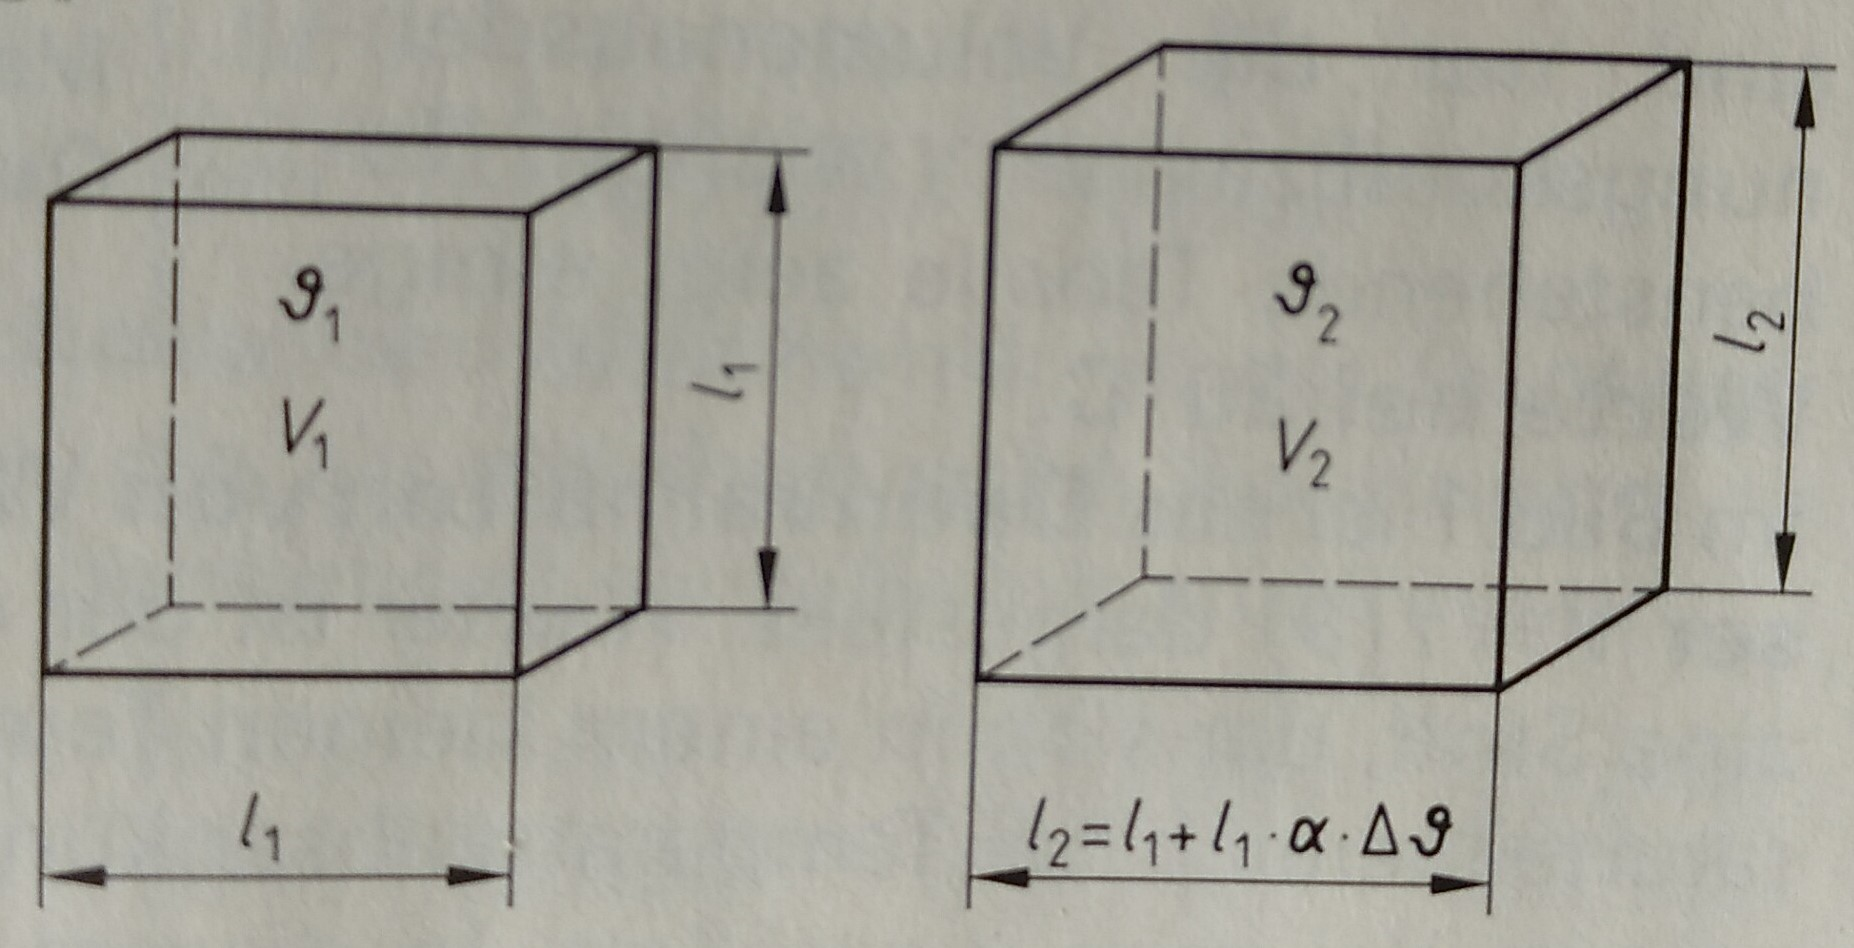
\includegraphics[width=1.2\linewidth]{Volumenausdehnung.jpg}
\end{wrapfigure}
Bei der thermischen Längenausdehnung dominiert eine Raumrichtung. Natürlich ist es auch so, dass sich der Körper in alle Raumrichtungen ausdehnt, und die Volumenausdehnung hat insbesondere bei kompakten Körpern bzw. Hohlkörpern Bedeutung. Hohlkörper (Gefäße) dehnen sich im gleichen Maß wie massive Körper (Vollkörper).\\
\textbf{bei $\vartheta_1$:} $V_1=l_1^{3}$; \textbf{bei $\vartheta_2$:} $V_2=l_2^{3}=(l_1+l_1\cdot\alpha\cdot\Delta\vartheta)^{3}=(l_1\cdot(1+\alpha\cdot\Delta\vartheta))^{3}=l_1^{3}\cdot(1+\alpha\cdot\Delta\vartheta)^{3}$\\
Nach Berechnung des kubischen Binoms $(1+\alpha\cdot\Delta\vartheta)^{3}$ ergibt sich:\\
$V_2=l_1^{3}\cdot(1+3\cdot\alpha\cdot\Delta\vartheta+3\cdot(\alpha\cdot\Delta\vartheta)^{2}+(\alpha\cdot\Delta\vartheta)^{3})\rightarrow$ \textbf{genaue Formel!}\\
\textbf{Näherung:} $V_2=l_1^{3}\cdot(1+3\cdot\alpha\cdot\Delta\vartheta)=l_1^{3}+l_1^{3}\cdot 3\cdot\alpha\cdot\Delta\vartheta$\\
Mit $l_1^{3}=V_1$ wird\\
$V_2=V_1+V_1\cdot 3\cdot\alpha\cdot\Delta\vartheta$
	\begin{block}{Berechnung der Volumenausdehnung infolge einer Temperaturdifferenz}
	\begin{align*}
	\gamma&=3\cdot\alpha &\rightarrow&\text{Volumenausdehnungskoeffizient}\\
	V_2&=V_1\pm V_1\cdot\gamma\cdot\Delta\vartheta &\rightarrow&\text{Endvolumen}
	\end{align*}
	\end{block}
	Die Einheit von $\gamma$ ist: $\frac{m^{3}}{m^{3}\cdot \si{\kelvin}}$
}

\frame
{
  \frametitle{Wärmeausdehnung von Flüssigkeiten}
  \begin{block}{}
  Wegen der geringen Kohäsionskräfte dehnen sich Flüssigkeiten bei Temperaturveränderung stärker als feste Körper aus. Da sie keine feste Form haben, sind nur die Volumenausdehnungskoeffizienten $\gamma$ wichtig.
  \end{block}
\textbf{Beispielaufgabe 2}\\
Welchen Raum nehmen $\SI{2,5}{\cubic\meter}$ Benzin von $\SI{10}{\celsius}$ nach der Erwärmung durch Sonneneinstrahlung auf eine Temperatur von $\SI{45}{\celsius}$ ein ($\gamma_{Benzin}=\SI{0.001}{\frac{\cubic\meter}{\cubic\meter\cdot\kelvin}}$)? Welche technische Regel leitet sich hieraus für die Aufbewahrung von Flüssigkeiten in geschlossenen Behältern ab?
}

\frame
{
\frametitle{Wärmeausdehnung von Flüssigkeiten}
\textbf{Lösung}\\
\begin{align*}
V_2&=V_1+ V_1\cdot\gamma\cdot\Delta\vartheta\\
V_2&=\SI{2,5}{\cubic\meter}+\SI{2,5}{\cubic\meter}\cdot\SI{0.001}{\frac{\cubic\meter}{\cubic\meter\cdot\kelvin}}\cdot\SI{35}{\kelvin}\\
&=\SI{2,5}{\cubic\meter}+\SI{0,0875}{\cubic\meter}=\SI{2,5875}{\cubic\meter}
\end{align*}
Das Volumen hat also um $\SI{87,5}{\liter}$ zugenommen!
}

\frame
{
\frametitle{Anomalie des Wassers}
	\begin{block}{Dehnverhalten von Wasser}
	Wasser hat bei $\SI{4}{\celsius}$ sein geringstes Volumen und damit seine größte Dichte $\varrho=\SI{1.00}{\kilo\gram\per\cubic\deci\meter}$.
	\end{block}
\begin{figure}
	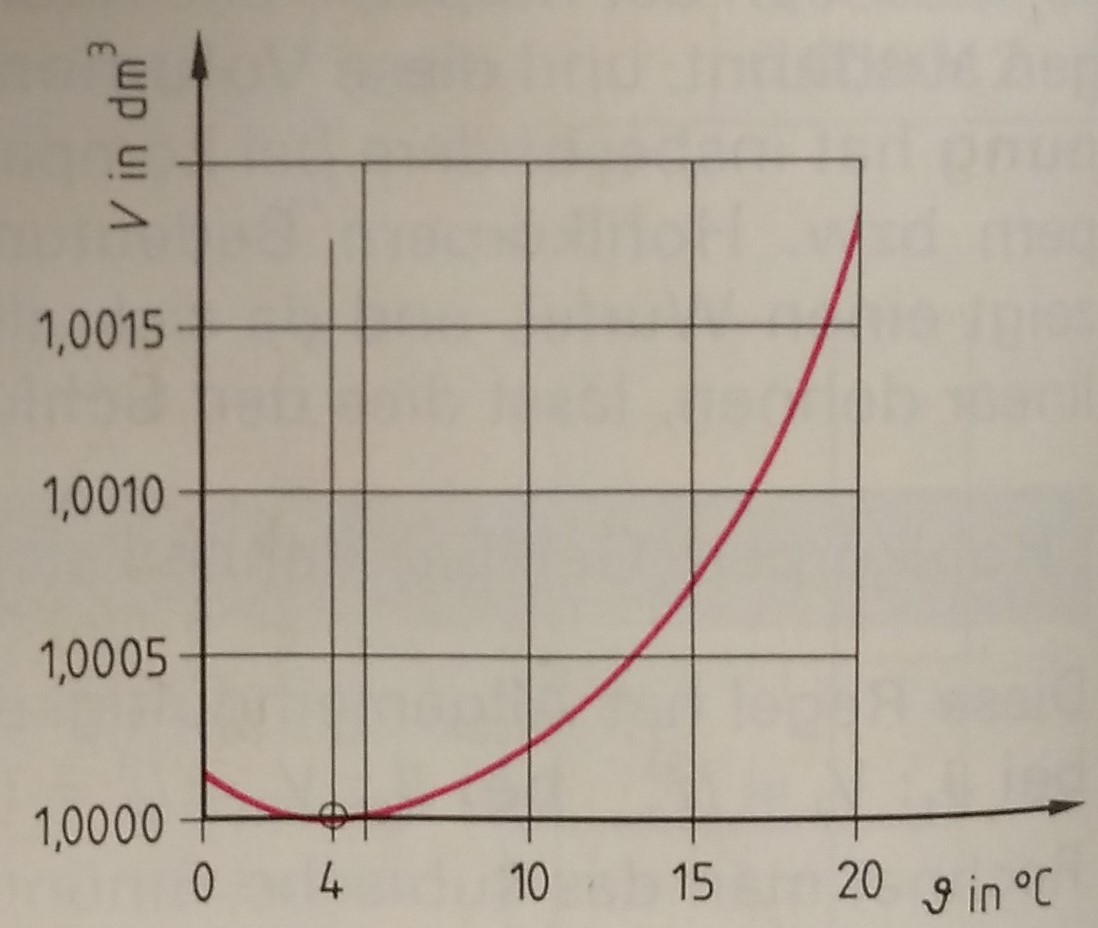
\includegraphics[width=0.5\linewidth]{Anomalie.jpg}
\end{figure}
}

\frame
{
\frametitle{Wärmespannung}
\begin{figure}
	\includegraphics[width=0.8\linewidth]{Wärmespannung.jpg}
\end{figure}
}

\frame
{
\frametitle{Wärmespannung}
	\begin{block}{elastische Verlängerung $\Delta l$}
	Die \textbf{elastische Verlängerung} $\Delta l$ eines Körpers ist der wirkenden Kraft $F$ proportional. (Hooke'sches Gesetz)\\
	Die elastische Verlängerung eines Körpers ist der Ausgangslänge $l_1$ proportional und der Querschnittsfläche $A$ umgekehrt proportional.
	$\Delta l\sim\dfrac{F\cdot l_1}{A}$
	\end{block}
	Eine Werkstoffkonstante, der \textbf{Elastizitätsmodul} $E$, berücksichtigt die Abhängigkeit vom verwendeten Werkstoff, und durch Versuche kann \textbf{im elastischen Bereich} bestätigt werden:\\
	$\Delta l=\dfrac{F\cdot l_1}{A\cdot E}$
}	
\frame
{
\frametitle{Wärmespannung}
	In der \textbf{Festigkeitslehre} ist der Quotient aus der Kraft $F$ und dem Querschnitt $A$ eine Größe, die als \textbf{mechanische Spannung} $\sigma$ z.B. \textbf{Zugspannung} $\sigma_z$ oder \textbf{Druckspannung} $\sigma_d$, bezeichnet wird.\\
	$\Delta l=\sigma\cdot\dfrac{l_1}{E}$\\
	nach Einsetzen der thermischen Längenausdehnung:\\
	$\Delta l=l_1\cdot\alpha\cdot\Delta\vartheta=\sigma\cdot\dfrac{l_1}{E}$\\
	Wärmespannung: $\sigma=E\cdot\alpha\cdot\Delta\vartheta$\\
	Zug- oder Druckkraft im Bauteil: $F=E\cdot\alpha\cdot\Delta\vartheta\cdot A$\\
	\begin{block}{}
	Die Wärmespannung und die daraus resultierende Zug- oder Druckkraft in einem Bauteil sind von der Bauteillänge unabhängig.
	\end{block}
}

\frame
{
\frametitle{Wärmespannung}
\begin{wrapfigure}{r}{3.5cm}
	\includegraphics[width=0.6\linewidth]{Wärmespannung.jpg}
\end{wrapfigure}
Die beiden Behälter im Bild sind mit einer Stahlrohrleitung mit dem Außendurchmesser $D=\SI{200}{\milli\meter}$ und dem Innendurchmesser $d=\SI{190}{\milli\meter}$ verbunden. Bei der verwendeten Stahlqualität kann von $E=\SI{215000}{\newton\per\square\milli\meter} $ und $\alpha=\SI{0.000012}{\meter\per\meter\per\kelvin}$ ausgegangen werden. Nach spannungsfreiem Einbau erwärmt sich die Leitung um $\Delta\vartheta=\SI{70}{\celsius}$. Wie groß ist die Druckkraft $F$ in der Leitung?\\
\textbf{Lösung:}
\begin{align*}
F&=E\cdot\alpha\cdot\Delta\vartheta\cdot A\\
A&=\dfrac{\pi}{4}\cdot(D^{2}-d^{2})=\dfrac{\pi}{4}\cdot(200^{2}-190^{2})\si{\square\milli\meter}=\SI{3063}{\square\milli\meter}\\
F&=\SI{215000}{\newton\per\square\milli\meter}\cdot\SI{0.000012}{\meter\per\meter\per\kelvin}\cdot\SI{70}{\kelvin}\cdot\SI{3063}{\square\milli\meter}\\
F&=\SI{553}{\kilo\newton}
\end{align*}
}
\end{document}
